\documentclass[11pt]{standalone}
\usepackage{amssymb}
\usepackage{amsmath}
\usepackage[no-math]{fontspec}
\usepackage{unicode-math}
\usepackage{libertinus}
\usepackage{pgf,xcolor}
\usepackage{tikz}
\usetikzlibrary{arrows.meta, backgrounds}
\usepackage{pgfplots}
\pgfplotsset{compat=newest}

\definecolor{my_darkgray}{HTML}{484949}
\definecolor{my_lightgray}{HTML}{F3F4F4}
\definecolor{my_darkblue}{HTML}{005A94}
\definecolor{my_lightblue}{HTML}{CCDEE9}
\definecolor{my_yellow}{HTML}{FFEC7F}
\definecolor{my_red}{HTML}{E60000}
\definecolor{my_orange}{HTML}{E87846}

\begin{document}
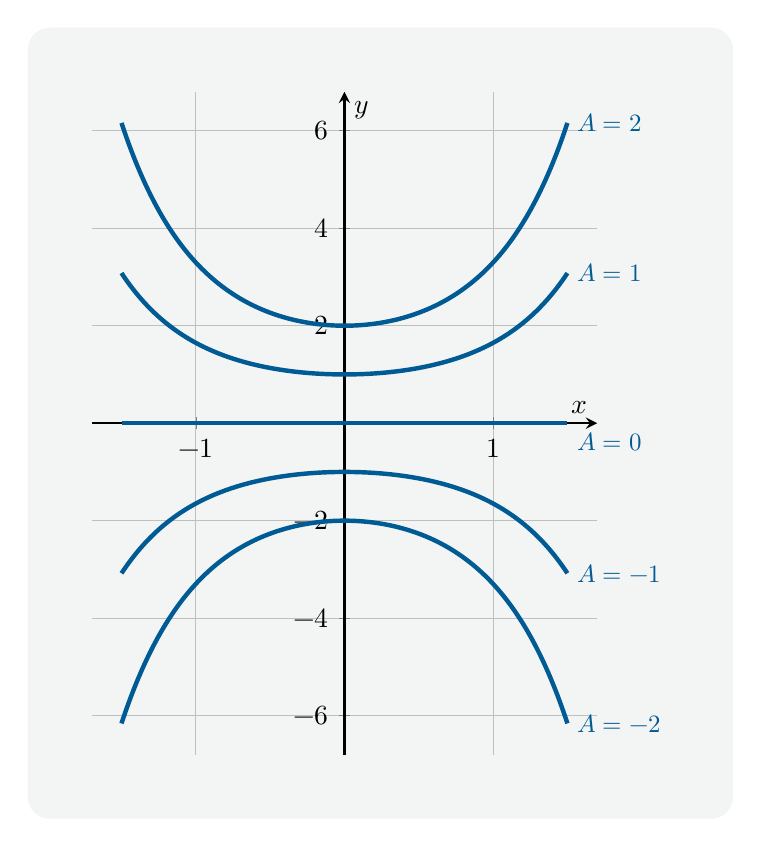
\begin{tikzpicture}[
    show background rectangle,
    background rectangle/.style={fill=my_lightgray, rounded corners=8pt},
    inner frame sep=0.8cm
]
% ---------------------------------------------------------------
%  Loesungen y = A e^{x^2/2} der DGL y' = x y fuer A = -2, ..., 2
%  Werte bei x = 1.5: e^{1.125} = 3.08, also +-3.08 und +-6.16
%  axis equal weggelassen: Bei gleicher Skalierung waere das Bild
%  bei y-Werten bis 6 und x-Werten bis 1.5 viermal so hoch wie breit.
% ---------------------------------------------------------------
\begin{axis}[
    axis lines = center,
    xlabel = {$x$},
    ylabel = {$y$},
    grid = both,
    axis line style={thick},
    width=8cm, height=10cm,
    xmin=-1.7, xmax=1.7,
    ymin=-6.8, ymax=6.8,
    xtick={-1, 1},
    ytick={-6, -4, -2, 2, 4, 6},
    clip=false,
]
\foreach \A in {-2, -1, 0, 1, 2}{
    \addplot[draw=my_darkblue, samples=300, ultra thick, domain=-1.5:1.5]
        {\A*exp(x^2/2)};
}
\node[right, font=\small, my_darkblue] at (axis cs:1.5, 6.16) {$A = 2$};
\node[right, font=\small, my_darkblue] at (axis cs:1.5, 3.08) {$A = 1$};
\node[below right, font=\small, my_darkblue] at (axis cs:1.5, 0) {$A = 0$};
\node[right, font=\small, my_darkblue] at (axis cs:1.5, -3.08) {$A = -1$};
\node[right, font=\small, my_darkblue] at (axis cs:1.5, -6.16) {$A = -2$};
\end{axis}
\end{tikzpicture}
\end{document}
